\title{Getting Started}

% Begin the content of the page
\subsection{Getting Started}
Getting started with Edward is easy.

\subsubsection{Quick Installation}
To install the latest stable version, run

\begin{lstlisting}[language=Java]
pip install edward
\end{lstlisting}

To install the latest development version, run

\begin{lstlisting}[language=Java]
pip install -e "git+https://github.com/blei-lab/edward.git#egg=edward"
\end{lstlisting}

See the \href{troubleshooting}{troubleshooting page} for detailed
installation instructions.


\subsubsection{Your first Edward program}

Probabilistic models are built in Edward using one of the available
modeling languages. Here we use TensorFlow to define a Bayesian neural
network: a neural network with a prior distribution on its weights.
(This example is abridged; full source
\href{https://github.com/blei-lab/edward/blob/master/examples/getting_started_example.py}
{here}.)
\begin{lstlisting}[language=Python]
import tensorflow as tf
from edward.stats import norm

class BayesianNN:
    """Bayesian neural network for regression"""
    def __init__(self, layer_sizes):
        self.layer_sizes = layer_sizes
        self.weight_dims = list(zip(layer_sizes[:-1], layer_sizes[1:]))
        self.n_vars = sum((m+1)*n for m, n in self.weight_dims)

    def log_prob(self, xs, zs):
        # Extract inputs/outputs from data `xs` and latent vars `zs`.
        x, y = xs['x'], xs['y']
        zs = zs['z']
        # Specify the prior on neural network weights `zs`.
        log_prior = tf.reduce_sum(norm.logpdf(zs, loc=0, scale=1), 1)
        # Specify the likelihood. Its mean is the output of a neural
        # network taking `x` as input with weights `zs`.
        mus = self.neural_network(x, zs)
        log_lik = tf.reduce_sum(norm.logpdf(y, loc=mus, scale=1), 1)
        return log_prior + log_lik
\end{lstlisting}

Instantiate this model as
\begin{lstlisting}[language=Python]
model = BayesianNN(layer_sizes=[1, 2, 2, 1])
\end{lstlisting}
This defines a two-layer Bayesian neural network with $\tanh$
nonlinearities.

First, simulate a toy dataset of 50 observations with a cosine relationship.
\begin{lstlisting}[language=Python]
import numpy as np

x = np.linspace(-3, 3, num=50)
y = np.cos(x) + norm.rvs(0, 0.1, size=50)
data = {'x': x, 'y': y}
\end{lstlisting}
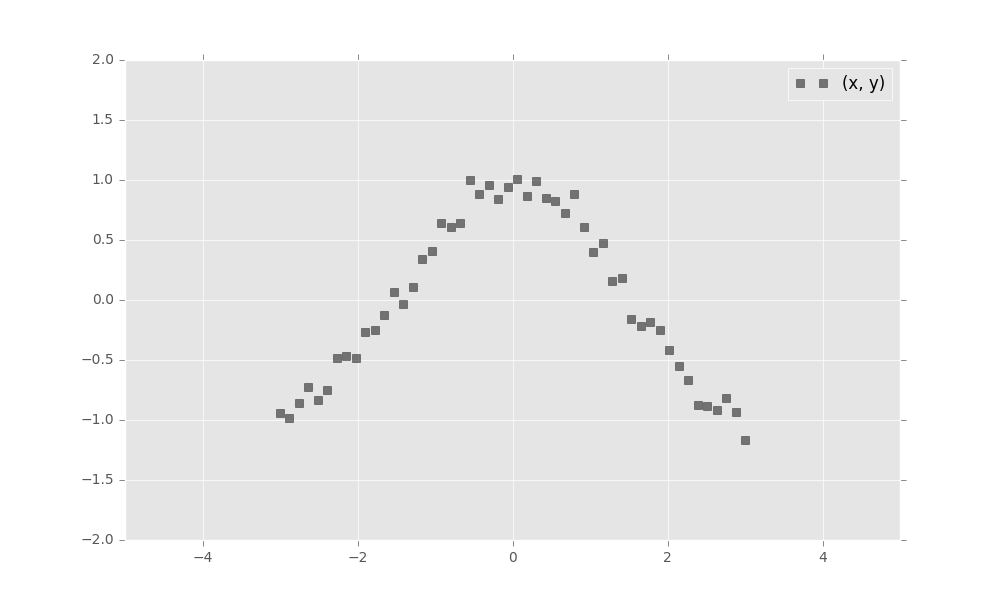
\includegraphics[width=700px]{images/getting-started-fig0.png}

Next, make inferences about the model from data.
Edward focuses on variational inference. Specify a mean-field normal
approximation as
\begin{lstlisting}[language=Python]
from edward.models import Normal

qz = Normal(model.n_vars)
\end{lstlisting}
The number of latent variables \texttt{model.n_vars} is the number
of weights and biases in the neural network.

Now, run mean-field variational inference. Infer the latent variable
\texttt{'z'} using \texttt{qz} conditional on the data (and model). We
specify \texttt{1000} iterations with a batch of \texttt{10}
datapoints per iteration.
\begin{lstlisting}[language=Python]
import edward as ed

inference = ed.MFVI({'z': qz}, data, model)
inference.run(n_iter=1000, n_minibatch=10)
\end{lstlisting}

Finally, criticize the model fit. Bayesian neural networks define a
distribution over neural networks, so let's do a graphical check. Draw
neural networks from the inferred model and visualize how well it
fits the data.

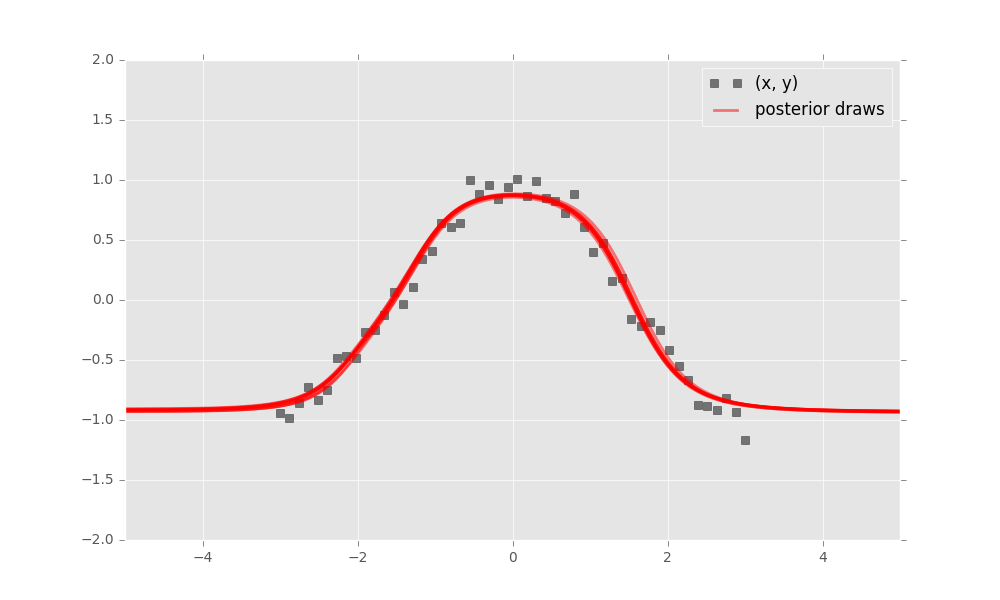
\includegraphics[width=700px]{images/getting-started-fig1.png}

The model has learned the cosine relationship between $x$ and $y$.

To learn more about Edward, \href{delving-in}{delve in}!

If you prefer to learn via examples, then check out some
\href{tutorials}{tutorials}.
